%%%%%%%%%%%%  v2.0.0-beta  %%%%%%%%%%%%%%

\documentclass[12pt]{report}
\usepackage{amsmath}
\usepackage{latexsym}
\usepackage{amsfonts}
\usepackage[normalem]{ulem}
\usepackage{array}
\usepackage{amssymb}
\usepackage{graphicx}
\usepackage[backend=biber,
style=numeric,
sorting=none,
isbn=false,
doi=false,
url=false,
]{biblatex}\addbibresource{bibliography.bib}

\usepackage{subfig}
\usepackage{wrapfig}
\usepackage{wasysym}
\usepackage{enumitem}
\usepackage{adjustbox}
\usepackage{ragged2e}
\usepackage[svgnames,table]{xcolor}
\usepackage{tikz}
\usepackage{longtable}
\usepackage{changepage}
\usepackage{setspace}
\usepackage{hhline}
\usepackage{multicol}
\usepackage{tabto}
\usepackage{float}
\usepackage{multirow}
\usepackage{makecell}
\usepackage{fancyhdr}
\usepackage[toc,page]{appendix}
\usepackage[hidelinks]{hyperref}
\usetikzlibrary{shapes.symbols,shapes.geometric,shadows,arrows.meta}
\tikzset{>={Latex[width=1.5mm,length=2mm]}}
\usepackage{flowchart}\usepackage[paperheight=11.0in,paperwidth=8.5in,left=1.0in,right=1.0in,top=1.0in,bottom=1.0in,headheight=1in]{geometry}
\usepackage[utf8]{inputenc}
\usepackage[T1]{fontenc}
\TabPositions{0.5in,1.0in,1.5in,2.0in,2.5in,3.0in,3.5in,4.0in,4.5in,5.0in,5.5in,6.0in,}

\urlstyle{same}


 %%%%%%%%%%%%  Set Depths for Sections  %%%%%%%%%%%%%%

% 1) Section
% 1.1) SubSection
% 1.1.1) SubSubSection
% 1.1.1.1) Paragraph
% 1.1.1.1.1) Subparagraph


\setcounter{tocdepth}{5}
\setcounter{secnumdepth}{5}


 %%%%%%%%%%%%  Set Depths for Nested Lists created by \begin{enumerate}  %%%%%%%%%%%%%%


\setlistdepth{9}
\renewlist{enumerate}{enumerate}{9}
		\setlist[enumerate,1]{label=\arabic*)}
		\setlist[enumerate,2]{label=\alph*)}
		\setlist[enumerate,3]{label=(\roman*)}
		\setlist[enumerate,4]{label=(\arabic*)}
		\setlist[enumerate,5]{label=(\Alph*)}
		\setlist[enumerate,6]{label=(\Roman*)}
		\setlist[enumerate,7]{label=\arabic*}
		\setlist[enumerate,8]{label=\alph*}
		\setlist[enumerate,9]{label=\roman*}

\renewlist{itemize}{itemize}{9}
		\setlist[itemize]{label=$\cdot$}
		\setlist[itemize,1]{label=\textbullet}
		\setlist[itemize,2]{label=$\circ$}
		\setlist[itemize,3]{label=$\ast$}
		\setlist[itemize,4]{label=$\dagger$}
		\setlist[itemize,5]{label=$\triangleright$}
		\setlist[itemize,6]{label=$\bigstar$}
		\setlist[itemize,7]{label=$\blacklozenge$}
		\setlist[itemize,8]{label=$\prime$}

\setlength{\topsep}{0pt}\setlength{\parskip}{8.04pt}
\setlength{\parindent}{0pt}

 %%%%%%%%%%%%  This sets linespacing (verticle gap between Lines) Default=1 %%%%%%%%%%%%%%


\renewcommand{\arraystretch}{1.3}


%%%%%%%%%%%%%%%%%%%% Document code starts here %%%%%%%%%%%%%%%%%%%%



\begin{document}


%%%%%%%%%%%%%%%%%%%% Figure/Image No: 1 starts here %%%%%%%%%%%%%%%%%%%%

\begin{figure}[H]
	\begin{Center}
		
\includegraphics[width=4.26in,height=0.95in]{./image1.jpg}
	\end{Center}
\end{figure}


%%%%%%%%%%%%%%%%%%%% Figure/Image No: 1 Ends here %%%%%%%%%%%%%%%%%%%%

\par


\vspace{\baselineskip}
\begin{Center}
{\fontsize{14pt}{16.8pt}\selectfont \textbf{\textcolor[HTML]{2F5496}{SOEN 6481}}\par}
\end{Center}\par

\begin{Center}
{\fontsize{14pt}{16.8pt}\selectfont \textbf{\textcolor[HTML]{2F5496}{SOFTWARE SYSTEMS REQUIREMENTS SPECIFICATION}}\par}
\end{Center}\par

\begin{Center}
{\fontsize{14pt}{16.8pt}\selectfont \textbf{\textcolor[HTML]{2F5496}{Summer 2019}}\par}
\end{Center}\par

\begin{Center}
{\fontsize{14pt}{16.8pt}\selectfont \textbf{\textcolor[HTML]{2F5496}{Project ETERNITY: NUMBERS- Deliverable 1}}\par}
\end{Center}\par

\begin{Center}
{\fontsize{14pt}{16.8pt}\selectfont \textbf{\textcolor[HTML]{2F5496}{Team-F}}\par}
\end{Center}\par


\vspace{\baselineskip}

\vspace{\baselineskip}

\vspace{\baselineskip}

\vspace{\baselineskip}

\vspace{\baselineskip}

\vspace{\baselineskip}
\begin{FlushRight}
\textbf{Submitted to: \textcolor[HTML]{2F5496}{P. Kamthan.}}
\end{FlushRight}\par

\begin{FlushRight}
\textbf{TA: \textcolor[HTML]{2F5496}{Mr. M.Ishanian}}
\end{FlushRight}\par

\begin{FlushRight}
\textbf{\textcolor[HTML]{2F5496}{ZINNIA RANA}}
\end{FlushRight}\par

\begin{FlushRight}
\textbf{\textcolor[HTML]{2F5496}{40074965}}
\end{FlushRight}\par


\vspace{\baselineskip}

\vspace{\baselineskip}

\vspace{\baselineskip}

\vspace{\baselineskip}

\vspace{\baselineskip}

\vspace{\baselineskip}

\vspace{\baselineskip}

\vspace{\baselineskip}

\vspace{\baselineskip}

\vspace{\baselineskip}

\vspace{\baselineskip}
\section*{Abstract}
\addcontentsline{toc}{section}{Abstract}

\vspace{\baselineskip}
\begin{justify}
The use of irrational numbers in the computational areas make this Eternity: Numbers calculator unique compared to the ones available in market. This calculator provides the functionality to compute the values of high-level mathematical equations by simply providing the functionality to the user to use irrational number values and feasibility to solve complex problems with number of predefined functions.
\end{justify}\par


\vspace{\baselineskip}
\begin{justify}
This report mainly focusses upon the requirement specifications related to this calculator and the important irrational numbers that we will be providing. The main goal was to attain well informed software requirements by conducting various activities.
\end{justify}\par


\vspace{\baselineskip}
\begin{justify}
In order to achieve this, I interviewed two prospective users who were aware of the \textbf{Eternity: Numbers}  i.e. Euler Number and analyzed their requirements and goals for what they will be using this feature for. They use it in some application areas, in their fields to solve calculations and attain certain goals which helped me a lot to comprehensive understand the business goals and value for the user simultaneously.
\end{justify}\par


\vspace{\baselineskip}
\begin{justify}
Furthermore, this gave me the basis for designing a domain model of the \textbf{Eternity: Numbers} calculator and come up with some use cases and their flow for \textbf{Eternity: Numbers}. Thus, it provided me the base to collectively sum up and represent my understanding using UML diagrams.
\end{justify}\par


\vspace{\baselineskip}

\vspace{\baselineskip}

\vspace{\baselineskip}

\vspace{\baselineskip}

\vspace{\baselineskip}

\vspace{\baselineskip}

\vspace{\baselineskip}

\vspace{\baselineskip}

\vspace{\baselineskip}

\vspace{\baselineskip}

\vspace{\baselineskip}

\vspace{\baselineskip}

\vspace{\baselineskip}
\section*{Acknowledgement}
\addcontentsline{toc}{section}{Acknowledgement}

\vspace{\baselineskip}
\begin{justify}
I would like to pay my regards to the Professor Pankaj Kamthan for his guidance and patience for clearing the doubts throughout the term. 
\end{justify}\par


\vspace{\baselineskip}
\begin{justify}
Furthermore, I would also like to sincerely thank my TA Mr. M. Ishanian for being patient and supportive and providing proper guidance towards the approach and being such flexible in helping out to all the extent. His expertise in providing interviews perspective understanding and Latex helped me a lot to achieve my project goal to the fullest. 
\end{justify}\par


\vspace{\baselineskip}
\begin{justify}
And lastly, I am thankful to all my teammates for cooperation with all the team activities and discussion about any concern regarding this project.
\end{justify}\par


\vspace{\baselineskip}

\vspace{\baselineskip}

\vspace{\baselineskip}

\vspace{\baselineskip}

\vspace{\baselineskip}

\vspace{\baselineskip}

\vspace{\baselineskip}

\vspace{\baselineskip}

\vspace{\baselineskip}

\vspace{\baselineskip}

\vspace{\baselineskip}

\vspace{\baselineskip}

\vspace{\baselineskip}

\vspace{\baselineskip}

\vspace{\baselineskip}

\vspace{\baselineskip}


 %%%%%%%%%%%%  This Produces Table Of Contents %%%%%%%%%%%%%%

\tableofcontents
\addcontentsline{toc}{chapter}{Contents}

\vspace{\baselineskip}

\vspace{\baselineskip}

\vspace{\baselineskip}

\vspace{\baselineskip}

\vspace{\baselineskip}

\vspace{\baselineskip}

\vspace{\baselineskip}

\vspace{\baselineskip}

\vspace{\baselineskip}

\vspace{\baselineskip}

\vspace{\baselineskip}

\vspace{\baselineskip}

\vspace{\baselineskip}

\vspace{\baselineskip}

\vspace{\baselineskip}
\begin{justify}
{\fontsize{14pt}{16.8pt}\selectfont \textbf{\textcolor[HTML]{2F5496}{Introduction:}}\par}
\end{justify}\par


\vspace{\baselineskip}
\begin{justify}
Euler Number is one of the unique irrational number, and is equally important among other popular numbers such as pi, discovered in early 18th century named after the Swiss mathematician Leonhard Euler. '\textit{e }'is considered as the base of natural logarithm and its natural log value is equal to one, and is often confused with Euler's constant. The first few digits are: 2.7182818284590452353602874713527.
\end{justify}\par

\begin{justify}
It is considered as the limit of :
\end{justify}\par

\begin{adjustwidth}{2.5in}{0.0in}
\textbf{(1 + 1/n)n}\par

\end{adjustwidth}

\begin{justify}
and as n increases it reaches the value of \textit{e}. 
\end{justify}\par

\begin{justify}
{\fontsize{14pt}{16.8pt}\selectfont \textbf{\textcolor[HTML]{2F5496}{Characteristics:}}\par}
\end{justify}\par

\begin{justify}
Its specific characteristic is it is considered as the limit to a sequence, and its usage in integral calculus for computations. Euler number is equals to the sum of infinite series and is used in the natural exponential function, where the slope on the graph is its value and also the area covered under the slope is calculated by e. The area up to any x-value is also equal to ex:
\end{justify}\par


\vspace{\baselineskip}


%%%%%%%%%%%%%%%%%%%% Figure/Image No: 2 starts here %%%%%%%%%%%%%%%%%%%%

\begin{figure}[H]
	\begin{Center}
		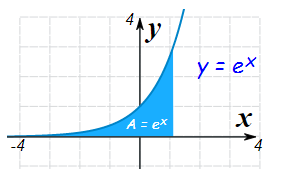
\includegraphics[width=3.05in,height=1.91in]{./image2.png}
	\end{Center}
\end{figure}


%%%%%%%%%%%%%%%%%%%% Figure/Image No: 2 Ends here %%%%%%%%%%%%%%%%%%%%

\par

\begin{justify}
{\fontsize{14pt}{16.8pt}\selectfont \textbf{\textcolor[HTML]{2F5496}{Applications:}}\par}
\end{justify}\par

\begin{justify}
This expression lead to foundation of compound interest known as \textbf{Napier's Constant}. \textit{e} is considered to be highly beneficial for continuously evolving process as is derived as the base of growth rate. It is commonly used in calculating probability in Bernoulli trials, Derangements and especially solving calculus.
\end{justify}\par


\vspace{\baselineskip}

\vspace{\baselineskip}

\vspace{\baselineskip}

\vspace{\baselineskip}

\vspace{\baselineskip}
\section*{Interviews}
\addcontentsline{toc}{section}{Interviews}

\vspace{\baselineskip}
\begin{justify}
I chose the interviewees having a strong mathematical background or enrolled in research in data science or working professionals. Few of them do not use calculator to that extent and the irrational numbers use in their field. Whereas , on the other hand one of the candidates did used the Euler number in Statistical analysis and solving theory computations. For example, the candidate had created his own word problem using it. The candidate is simultaneously working on a research project of physics which requires complex analysis and calculations with mathematical proof. 
\end{justify}\par


\vspace{\baselineskip}
\subsection*{Interview Questions:}
\addcontentsline{toc}{subsection}{Interview Questions:}

\vspace{\baselineskip}
\setstretch{2.0}
\begin{enumerate}
	\item Which age group describes you? \par

	\item What is the highest degree or level of school you have completed or currently pursuing?\par

	\item Do you use calculator in your daily use? If yes, then please answer the following questions.\par

	\item Are you aware of Euler's Number?\par

	\item Where do you use Euler's Number?\par

	\item Do you use any other Irrational Number/constant with this number? If yes then please mention.\par

	\item Will you be interested to use a calculator with irrational number functionality?\par

	\item For what application will you use this calculator?\par

	\item What interface would you like to use for the application?
\end{enumerate}\par


\vspace{\baselineskip}

\vspace{\baselineskip}

\vspace{\baselineskip}

\vspace{\baselineskip}

\vspace{\baselineskip}

\vspace{\baselineskip}

\vspace{\baselineskip}

\vspace{\baselineskip}

\vspace{\baselineskip}
\subsection*{Interview 1}
\addcontentsline{toc}{subsection}{Interview 1}

\vspace{\baselineskip}
\begin{enumerate}
	\item Which age group describes you?\par

Answer: 18 to 29\par

	\item What is the highest degree or level of school you have completed or currently pursuing?\par

Answer: Graduate\par

	\item Do you use calculator in your daily use? If yes, then please answer the following questions.\par

Answer: Sometimes\par

	\item Are you aware of Euler's Number?\par

Answer: Yes\par

	\item Where do you use Euler's Number?\par

Answer: Solving mathematical theory questions, statistical analysis\par

	\item Do you use any other Irrational Number/constant with this number? If yes then please mention.\par

Answer: Pi, tau, i\par

	\item Will you be interested to use a calculator with irrational number functionality?\par

Answer: Yes\par

	\item For what application will you use this calculator?\par

Answer: Mathematical proofs\par

	\item What interface would you like to use for the application?
\end{enumerate}\par

Answer: Mobile Application\par


\vspace{\baselineskip}
\setstretch{1.0}
{\fontsize{14pt}{16.8pt}\selectfont \textbf{\textcolor[HTML]{2F5496}{Analysis: }}\par}The candidate has a good knowledge of using Euler’s formula and uses its application frequently in mathematical and statistical analysis of her research area in electronics. The candidate has a positive attitude towards having irrational number functionality in the calculator. \par


\vspace{\baselineskip}

\vspace{\baselineskip}

\vspace{\baselineskip}

\vspace{\baselineskip}

\vspace{\baselineskip}

\vspace{\baselineskip}

\vspace{\baselineskip}

\vspace{\baselineskip}

\vspace{\baselineskip}

\vspace{\baselineskip}

\vspace{\baselineskip}

\vspace{\baselineskip}

\vspace{\baselineskip}

\vspace{\baselineskip}

\vspace{\baselineskip}

\vspace{\baselineskip}

\vspace{\baselineskip}

\vspace{\baselineskip}

\vspace{\baselineskip}

\vspace{\baselineskip}

\vspace{\baselineskip}

\vspace{\baselineskip}

\vspace{\baselineskip}

\vspace{\baselineskip}

\vspace{\baselineskip}
\subsection*{Interview 2}
\addcontentsline{toc}{subsection}{Interview 2}

\vspace{\baselineskip}
\begin{enumerate}
	\item Which age group describes you?\par

Answer: 18 to 29 \par

	\item What is the highest degree or level of school you have completed or currently pursuing?\par

Answer: Graduate\par

	\item Do you use calculator in your daily use? If yes, then please answer the following questions.\par

Answer: Yes\par

	\item Are you aware of Euler's Number?\par

Answer: No\par

	\item Where do you use Euler's Number?\par

Answer: \par

	\item Do you use any other Irrational Number/constant with this number? If yes then please mention.\par

Answer: \par

	\item Will you be interested to use a calculator with irrational number functionality?\par

Answer: Yes\par

	\item For what application will you use this calculator?\par

Answer: May be somewhere in the data science field.\par

	\item What interface would you like to use for the application?
\end{enumerate}\par

Answer: Mobile Application\par


\vspace{\baselineskip}
{\fontsize{14pt}{16.8pt}\selectfont{{Analysis:\par}} }The candidate has no knowledge of Euler’s formula, but has a positive attitude towards learning it, so that he can use this extensive irrational no. calculation into his data science field.\par


\vspace{\baselineskip}

\vspace{\baselineskip}

\vspace{\baselineskip}

\vspace{\baselineskip}

\vspace{\baselineskip}

\vspace{\baselineskip}

\vspace{\baselineskip}

\vspace{\baselineskip}

\vspace{\baselineskip}

\vspace{\baselineskip}

\vspace{\baselineskip}

\vspace{\baselineskip}
\section*{Persona 1}
\addcontentsline{toc}{section}{Persona 1}

\vspace{\baselineskip}


%%%%%%%%%%%%%%%%%%%% Table No: 1 starts here %%%%%%%%%%%%%%%%%%%%


\begin{table}[H]
 			\centering
\begin{tabular}{p{1.86in}p{4.23in}}
\hline
%row no:1
\multicolumn{1}{|p{1.86in}}{{\fontsize{10pt}{12.0pt}\selectfont \textbf{Photo}} \par {\fontsize{10pt}{12.0pt}\selectfont \textbf{\ \ \ \ \   }} \par 
	\begin{Center}
		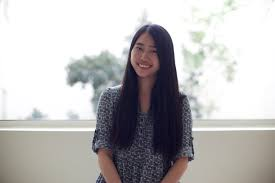
\includegraphics[width=1.86in,height=1.25in]{./image3.jpeg}
	\end{Center}
 \par } & 
\multicolumn{1}{|p{4.23in}|}{{\fontsize{10pt}{12.0pt}\selectfont \textbf{Private Information}} \par \begin{itemize}
	\item {\fontsize{10pt}{12.0pt}\selectfont Hina Advani} \par 	\item {\fontsize{10pt}{12.0pt}\selectfont Research Assistant} \par 	\item {\fontsize{10pt}{12.0pt}\selectfont 27} \par 	\item {\fontsize{10pt}{12.0pt}\selectfont Canada} \par 
\end{itemize}} \\
\hhline{--}
%row no:2
\multicolumn{2}{|p{6.29in}|}{{\fontsize{10pt}{12.0pt}\selectfont \textbf{Skills}} \par \begin{itemize}
	\item {\fontsize{10pt}{12.0pt}\selectfont Technology friendly } \par 	\item {\fontsize{10pt}{12.0pt}\selectfont Quick Learner} \par 	\item {\fontsize{10pt}{12.0pt}\selectfont Excellent Research Skills} \par 
\end{itemize}} \\
\hhline{--}
%row no:3
\multicolumn{2}{|p{6.29in}|}{{\fontsize{10pt}{12.0pt}\selectfont \textbf{Experience}} \par \begin{itemize}
	\item {\fontsize{10pt}{12.0pt}\selectfont Research assistant in Mcgill Lab in Electronics and Computer Science}
\end{itemize} \par } \\
\hhline{--}
%row no:4
\multicolumn{2}{|p{6.29in}|}{{\fontsize{10pt}{12.0pt}\selectfont \textbf{User requirements}} \par \begin{itemize}
	\item {\fontsize{10pt}{12.0pt}\selectfont Solve irrational number computations to perform complex analysis } \par 	\item {\fontsize{10pt}{12.0pt}\selectfont Statistical Analysis Computations} \par 	\item {\fontsize{10pt}{12.0pt}\selectfont Desktop Application} \par 
\end{itemize}} \\
\hhline{--}
%row no:5
\multicolumn{2}{|p{6.29in}|}{{\fontsize{10pt}{12.0pt}\selectfont \textbf{Goals}} \par {\fontsize{10pt}{12.0pt}\selectfont She wants the calculator with irrational numbers to solve mathematical proof calculations which can help her in her research area. } \par } \\
\hhline{--}

\end{tabular}
 \end{table}


%%%%%%%%%%%%%%%%%%%% Table No: 1 ends here %%%%%%%%%%%%%%%%%%%%


\vspace{\baselineskip}

\vspace{\baselineskip}

\vspace{\baselineskip}

\vspace{\baselineskip}

\vspace{\baselineskip}

\vspace{\baselineskip}

\vspace{\baselineskip}
\section*{Persona 2}
\addcontentsline{toc}{section}{Persona 2}

\vspace{\baselineskip}


%%%%%%%%%%%%%%%%%%%% Table No: 2 starts here %%%%%%%%%%%%%%%%%%%%


\begin{table}[H]
 			\centering
\begin{tabular}{p{1.86in}p{4.23in}}
\hline
%row no:1
\multicolumn{1}{|p{1.86in}}{{\fontsize{10pt}{12.0pt}\selectfont \textbf{Photo}} \par 
	\begin{Center}
		
\includegraphics[width=1.86in,height=1.11in]{./image4.jpeg}
	\end{Center}
{\fontsize{10pt}{12.0pt}\selectfont \textbf{\ \ \ \ \   }} \par } & 
\multicolumn{1}{|p{4.23in}|}{{\fontsize{10pt}{12.0pt}\selectfont \textbf{Private Information}} \par \begin{itemize}
	\item {\fontsize{10pt}{12.0pt}\selectfont Adam} \par 	\item {\fontsize{10pt}{12.0pt}\selectfont Graduate Student} \par 	\item {\fontsize{10pt}{12.0pt}\selectfont 24} \par 	\item {\fontsize{10pt}{12.0pt}\selectfont Australia}
\end{itemize} \par } \\
\hhline{--}
%row no:2
\multicolumn{2}{|p{6.29in}|}{{\fontsize{10pt}{12.0pt}\selectfont \textbf{Skills}} \par \begin{itemize}
	\item {\fontsize{10pt}{12.0pt}\selectfont Great Analysis skills} \par 	\item {\fontsize{10pt}{12.0pt}\selectfont Expertise Hadoop and Big-Data} \par 	\item {\fontsize{10pt}{12.0pt}\selectfont Expertise in User Interaction} \par 
\end{itemize}} \\
\hhline{--}
%row no:3
\multicolumn{2}{|p{6.29in}|}{{\fontsize{10pt}{12.0pt}\selectfont \textbf{Experience}} \par \begin{itemize}
	\item {\fontsize{10pt}{12.0pt}\selectfont 2 years of industrial experience in Software Production} \par 	\item {\fontsize{10pt}{12.0pt}\selectfont Research assistant in Computer Science\textbf{ }} \par 
\end{itemize}} \\
\hhline{--}
%row no:4
\multicolumn{2}{|p{6.29in}|}{{\fontsize{10pt}{12.0pt}\selectfont \textbf{User requirements}} \par \begin{itemize}
	\item {\fontsize{10pt}{12.0pt}\selectfont The user has no knowledge of working with Euler’s formula but might require in future.} \par 	\item {\fontsize{10pt}{12.0pt}\selectfont The user has learning requirement of mathematics in his application projects with big data technology and might need the use of irrational numbers computation.}
\end{itemize} \par } \\
\hhline{--}
%row no:5
\multicolumn{2}{|p{6.29in}|}{{\fontsize{10pt}{12.0pt}\selectfont \textbf{Goals}} \par {\fontsize{10pt}{12.0pt}\selectfont The interviewee would like to use this as a mobile application. Though he does not use the Eternity: Numbers but would like to use it in calculation evolved in big data research.} \par } \\
\hhline{--}

\end{tabular}
 \end{table}


%%%%%%%%%%%%%%%%%%%% Table No: 2 ends here %%%%%%%%%%%%%%%%%%%%


\vspace{\baselineskip}

\vspace{\baselineskip}

\vspace{\baselineskip}

\vspace{\baselineskip}

\vspace{\baselineskip}

\vspace{\baselineskip}

\vspace{\baselineskip}

\vspace{\baselineskip}

\vspace{\baselineskip}
\section*{Domain Model}
\addcontentsline{toc}{section}{Domain Model}

\vspace{\baselineskip}


%%%%%%%%%%%%%%%%%%%% Figure/Image No: 3 starts here %%%%%%%%%%%%%%%%%%%%

\begin{figure}[H]
	\begin{Center}
		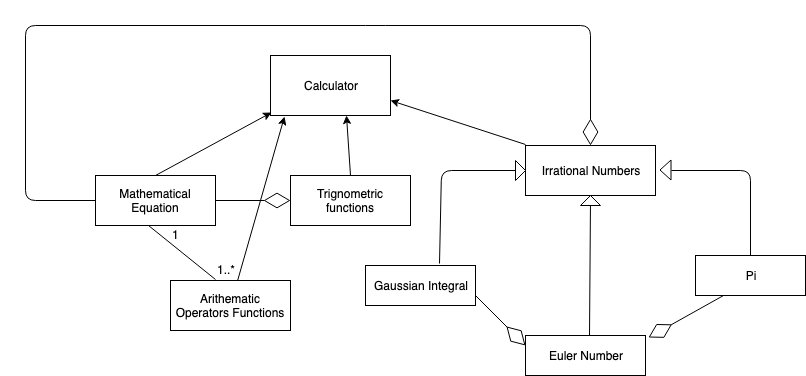
\includegraphics[width=7.1in,height=3.31in]{./image5.png}
	\end{Center}
\end{figure}


%%%%%%%%%%%%%%%%%%%% Figure/Image No: 3 Ends here %%%%%%%%%%%%%%%%%%%%

\par


\vspace{\baselineskip}

\vspace{\baselineskip}

\vspace{\baselineskip}

\vspace{\baselineskip}

\vspace{\baselineskip}

\vspace{\baselineskip}

\vspace{\baselineskip}

\vspace{\baselineskip}

\vspace{\baselineskip}

\vspace{\baselineskip}

\vspace{\baselineskip}

\vspace{\baselineskip}

\vspace{\baselineskip}
\section*{Use Case Model Views}
\addcontentsline{toc}{section}{Use Case Model Views}

\vspace{\baselineskip}
\subsection*{Use Case 1:}
\addcontentsline{toc}{subsection}{Use Case 1:}

\vspace{\baselineskip}

\vspace{\baselineskip}


%%%%%%%%%%%%%%%%%%%% Figure/Image No: 4 starts here %%%%%%%%%%%%%%%%%%%%

\begin{figure}[H]
	\begin{Center}
		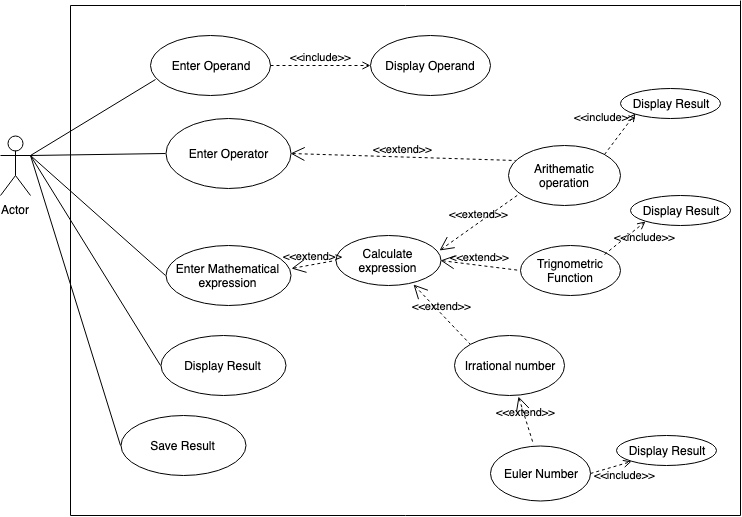
\includegraphics[width=7.07in,height=4.93in]{./image6.png}
	\end{Center}
\end{figure}


%%%%%%%%%%%%%%%%%%%% Figure/Image No: 4 Ends here %%%%%%%%%%%%%%%%%%%%

\par


\vspace{\baselineskip}

\vspace{\baselineskip}

\vspace{\baselineskip}

\vspace{\baselineskip}

\vspace{\baselineskip}

\vspace{\baselineskip}
\subsection*{Use Case 2:}
\addcontentsline{toc}{subsection}{Use Case 2:}

\vspace{\baselineskip}


%%%%%%%%%%%%%%%%%%%% Figure/Image No: 5 starts here %%%%%%%%%%%%%%%%%%%%

\begin{figure}[H]
	\begin{Center}
		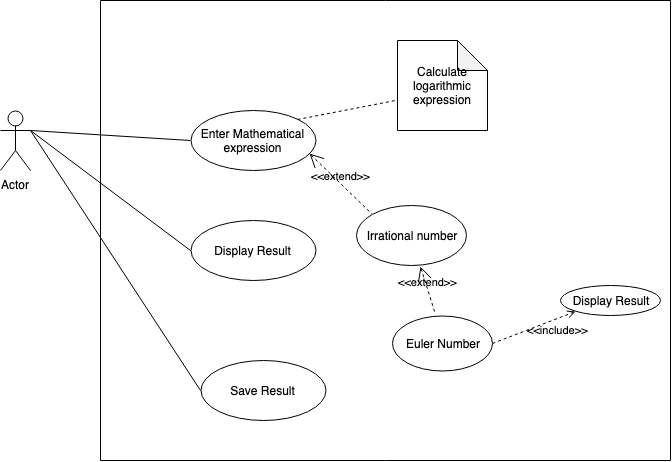
\includegraphics[width=7.12in,height=4.9in]{./image7.png}
	\end{Center}
\end{figure}


%%%%%%%%%%%%%%%%%%%% Figure/Image No: 5 Ends here %%%%%%%%%%%%%%%%%%%%

\par


\vspace{\baselineskip}

\vspace{\baselineskip}

\vspace{\baselineskip}

\vspace{\baselineskip}

\vspace{\baselineskip}

\vspace{\baselineskip}

\vspace{\baselineskip}
\section*{Scenario of Use Case Diagrams}
\addcontentsline{toc}{section}{Scenario of Use Case Diagrams}

\vspace{\baselineskip}
\subsection*{Scenario 1:}
\addcontentsline{toc}{subsection}{Scenario 1:}

\vspace{\baselineskip}


%%%%%%%%%%%%%%%%%%%% Figure/Image No: 6 starts here %%%%%%%%%%%%%%%%%%%%

\begin{figure}[H]
	\begin{Center}
		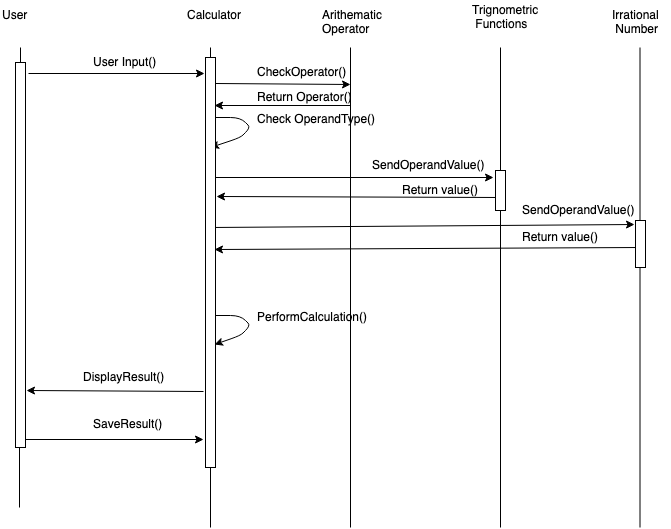
\includegraphics[width=7.0in,height=5.52in]{./image8.png}
	\end{Center}
\end{figure}


%%%%%%%%%%%%%%%%%%%% Figure/Image No: 6 Ends here %%%%%%%%%%%%%%%%%%%%

\par


\vspace{\baselineskip}

\vspace{\baselineskip}

\vspace{\baselineskip}

\vspace{\baselineskip}

\vspace{\baselineskip}

\vspace{\baselineskip}
\subsection*{Scenario 2:}
\addcontentsline{toc}{subsection}{Scenario 2:}

\vspace{\baselineskip}


%%%%%%%%%%%%%%%%%%%% Figure/Image No: 7 starts here %%%%%%%%%%%%%%%%%%%%

\begin{figure}[H]
	\begin{Center}
		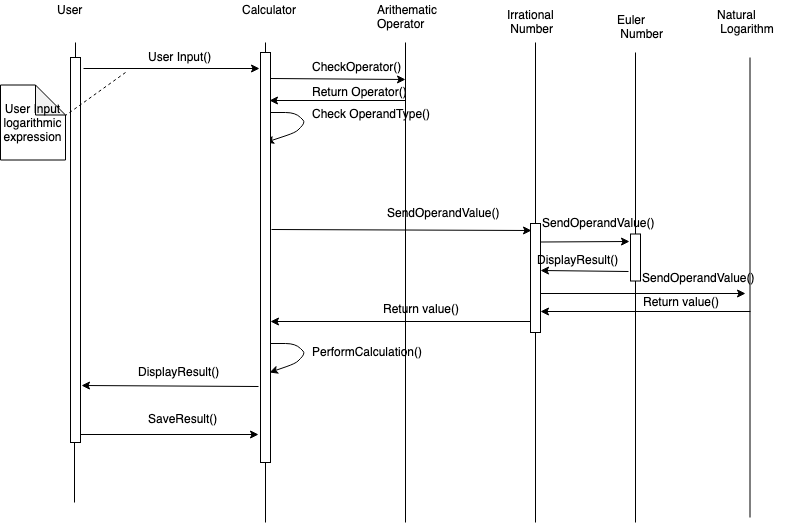
\includegraphics[width=7.22in,height=4.81in]{./image9.png}
	\end{Center}
\end{figure}


%%%%%%%%%%%%%%%%%%%% Figure/Image No: 7 Ends here %%%%%%%%%%%%%%%%%%%%

\par


\vspace{\baselineskip}

\vspace{\baselineskip}

\vspace{\baselineskip}

\vspace{\baselineskip}

\vspace{\baselineskip}

\vspace{\baselineskip}

\vspace{\baselineskip}

\vspace{\baselineskip}
\section*{Activity Diagram}
\addcontentsline{toc}{section}{Activity Diagram}

\vspace{\baselineskip}


%%%%%%%%%%%%%%%%%%%% Figure/Image No: 8 starts here %%%%%%%%%%%%%%%%%%%%

\begin{figure}[H]
	\begin{Center}
		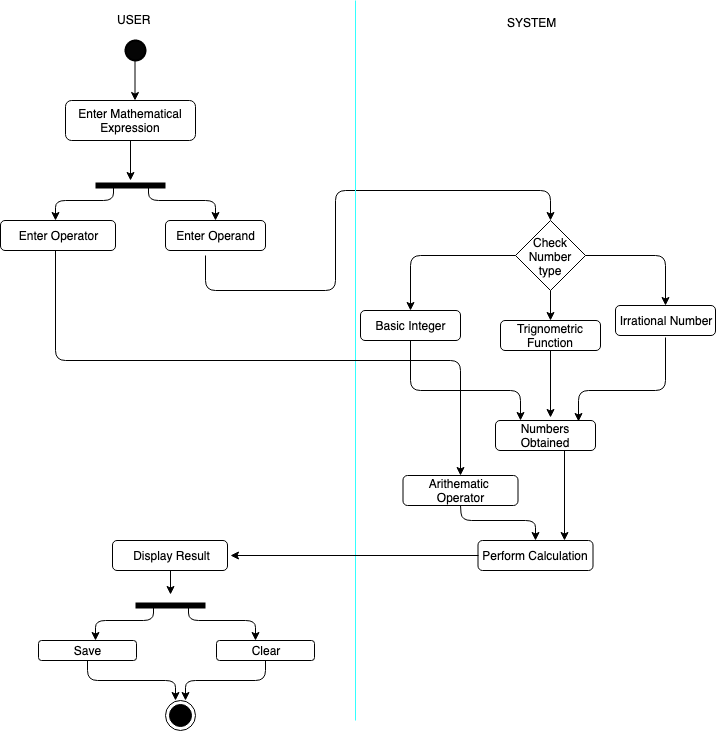
\includegraphics[width=6.5in,height=6.64in]{./image10.png}
	\end{Center}
\end{figure}


%%%%%%%%%%%%%%%%%%%% Figure/Image No: 8 Ends here %%%%%%%%%%%%%%%%%%%%

\par


\vspace{\baselineskip}

\vspace{\baselineskip}

\vspace{\baselineskip}

\vspace{\baselineskip}

\vspace{\baselineskip}

\vspace{\baselineskip}
\begin{itemize}
	\item \href{https://en.wikipedia.org/wiki/E_(mathematical_constant)}{https://en.wikipedia.org/wiki/E\_(mathematical\_constant)}\par

	\item \href{https://www.mathsisfun.com/numbers/e-eulers-number.html}{https://www.mathsisfun.com/numbers/e-eulers-number.html}\par

	\item \href{https://www.popularmechanics.com/science/math/a24383/mathematical-constant-e/}{https://www.popularmechanics.com/science/math/a24383/mathematical-constant-e/}\par

	\item \href{https://www.quora.com/Whats-so-special-about-the-Euler-number-e}{https://www.quora.com/Whats-so-special-about-the-Euler-number-e}\par

	\item \href{https://www.reddit.com/r/explainlikeimfive/comments/3u40tp/eli5_why_does_eulers_number_e_have_so_many_unique/}{https://www.reddit.com/r/explainlikeimfive/comments/3u40tp/eli5\_why\_does\_eulers\_number\_e\_have\_so\_many\_unique/}\par

	\item \href{https://math.stackexchange.com/questions/3092340/why-is-eulers-number-2-71828-and-not-anything-else}{https://math.stackexchange.com/questions/3092340/why-is-eulers-number-2-71828-and-not-anything-else}
\end{itemize}\par


\vspace{\baselineskip}

\end{document}